\documentclass[UTF8]{ctexart}
\usepackage{graphicx}
\usepackage{listings}
\usepackage{float}
\usepackage{subfigure}

\title{实验八报告}
\author{唐灵\\519030910052\\F1903002}
\date{\today}
\begin{document}
    \maketitle
    \begin{abstract}
        这是电工导c课程的第七次实验
    \end{abstract}
    \section{实验概览}
        本次实验主要应用cv2对于原始图片进读取,利用numpy对于我们希望得到的图片的基本特征进行处理以及抽取
        ,最终利用plt对于我们提取到的特征进行可视化。
    \section{实验环境}
    本次实验的所有代码在电类工程导论c课程中在课程方统一给定的“ee208”$Docker$容器中运行并实现。
    \section{练习解决思路}
        \subsection{练习一的解决思路}
            练习一要求作出RGB直方图,选择读取图像过后,将先将图片转化为RGB通道的图片。
            直接统计三个通道的总和,计算频率,可以简单通过numpy函数的sum函数得到:
            \begin{figure}[H]
                \centering
                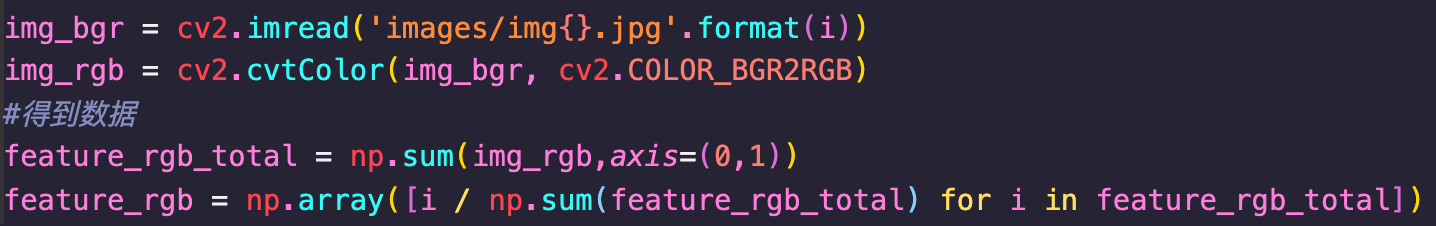
\includegraphics[scale=0.4]{img/RGB.png}
                \caption{得到RGB频数信息}
            \end{figure}

            之后再使用plt作直方图即可,值得注意的是应该考虑设定相当的颜色。
        \subsection{练习二的解决思路}
            练习二首先要求,读取灰度图,这个过程可以直接通过cv2实现,为方便作出频率直方图(plt.hist函数只能处理一维的narray数据),所以无论是在
            作梯度图还是在作灰度直方图的时候,都应该考虑将二维的图片“压”为一维的数组。\par
            对于灰度图直接作图即可,对于hist参数的选定,多考虑一下,比如归一化,将区间设定为整数等等。
            \begin{figure}[H]
                \centering
                
\includegraphics[scale=0.6]{img/gray.png}
                \caption{作灰度直方图}
            \end{figure}

            而对于梯度直方图而言,必须对于图片本身进行处理,我的处理方式分三个步骤:
            \begin{enumerate}
                \item 首先必须先对于图片本身的数据类型进行强制转化,因为cv2默认读取进来的是非负整型,没有办法进行接下来的运算
                \item 通过两个循环体,每个循环体的每一次循环将计算一行或者一列元素的梯度
                \item 将计算出的梯度放到列表中,最后再次转化为narray对象,
                \item 将对象的边缘进行切割,去除我们不需要的部分
                \item 其中列方向显然需要进行转置,才能进行下一步的处理
                \item 将两个方向分别得到的梯度图像进行平方和并开方的处理,得到最终的梯度图像
            \end{enumerate}

            最终的实际的代码相对来说还是比较简洁:
            \begin{figure}[H]
                \centering
                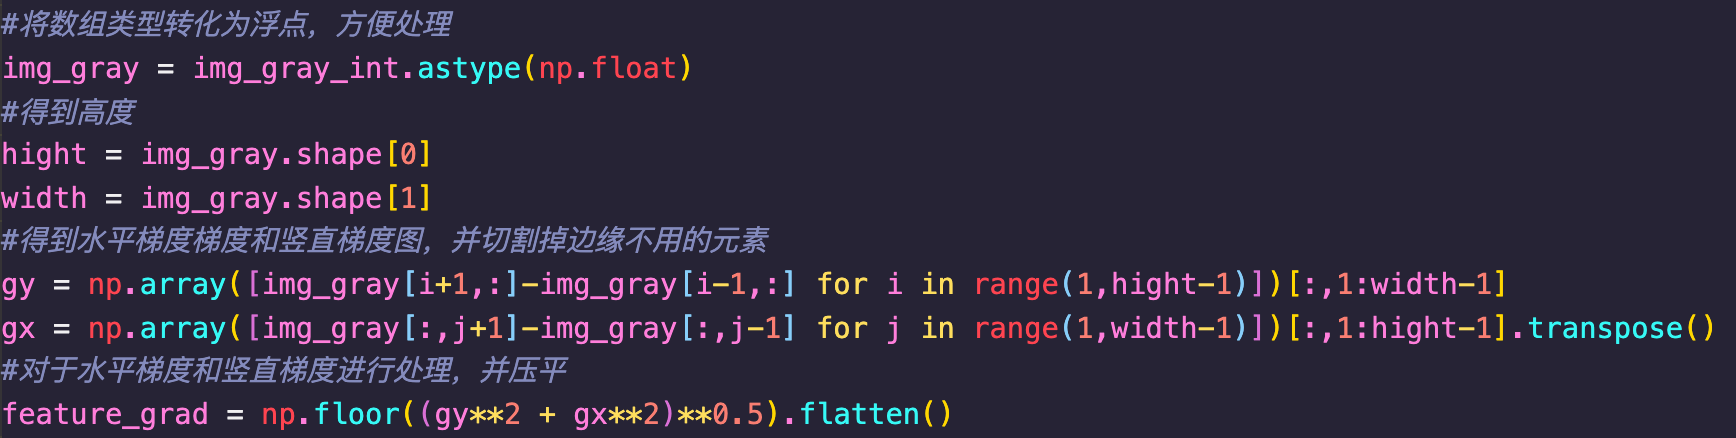
\includegraphics[scale=0.35]{img/grad.png}
                \caption{提取梯度信息}
            \end{figure}

    \section{代码运行结果}
        \subsection{练习一的运行结果}
            \begin{figure}[H]
                \centering
                \subfigure[img1-原图]{
                \begin{minipage}[t]{0.5\linewidth}
                \centering
                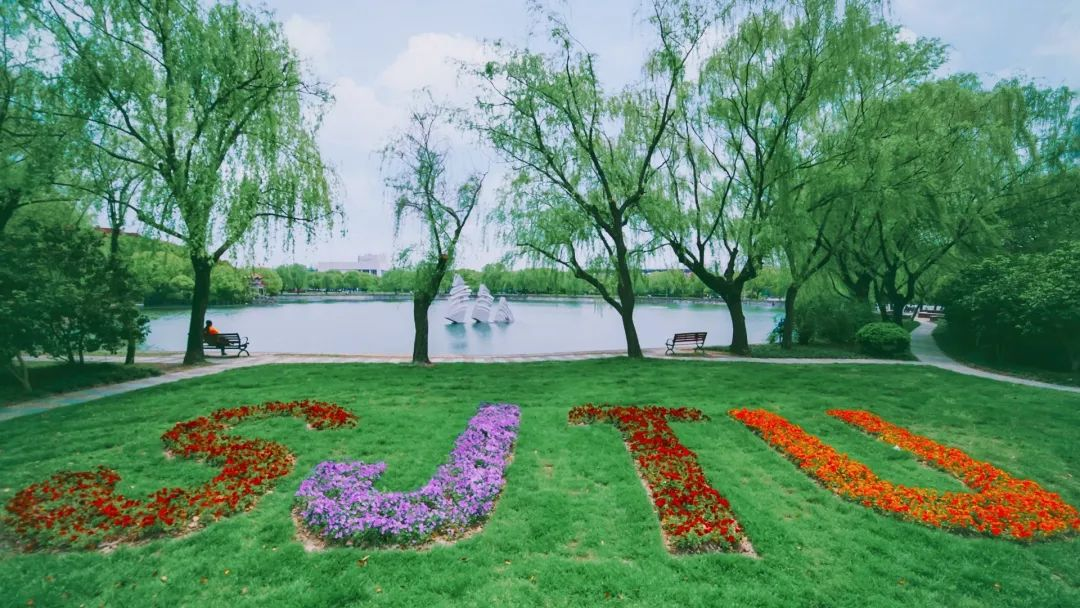
\includegraphics[width=1.5in]{img/images/img1.jpg}
                %\caption{fig1}
                \end{minipage}%
                }%
                \centering
                \subfigure[img1-RGB直方图]{
                \begin{minipage}[t]{0.5\linewidth}
                \centering
                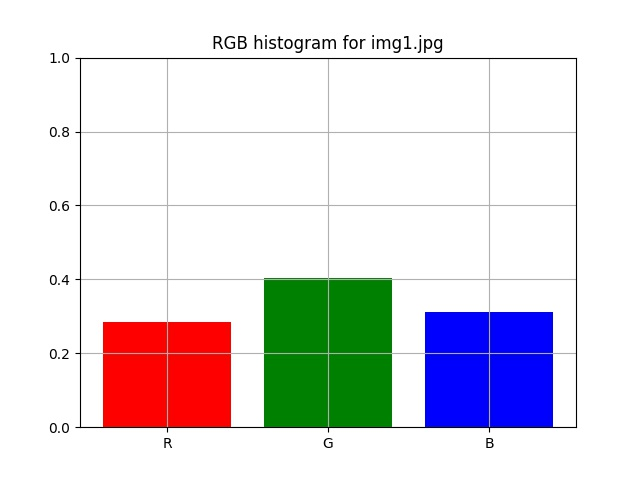
\includegraphics[width=1.5in]{img/feature/color/img1.jpg}
                %\caption{fig1}
                \end{minipage}%
                }%
            \end{figure}
            \begin{figure}[H]
                \centering
                \subfigure[img2-原图]{
                \begin{minipage}[t]{0.5\linewidth}
                \centering
                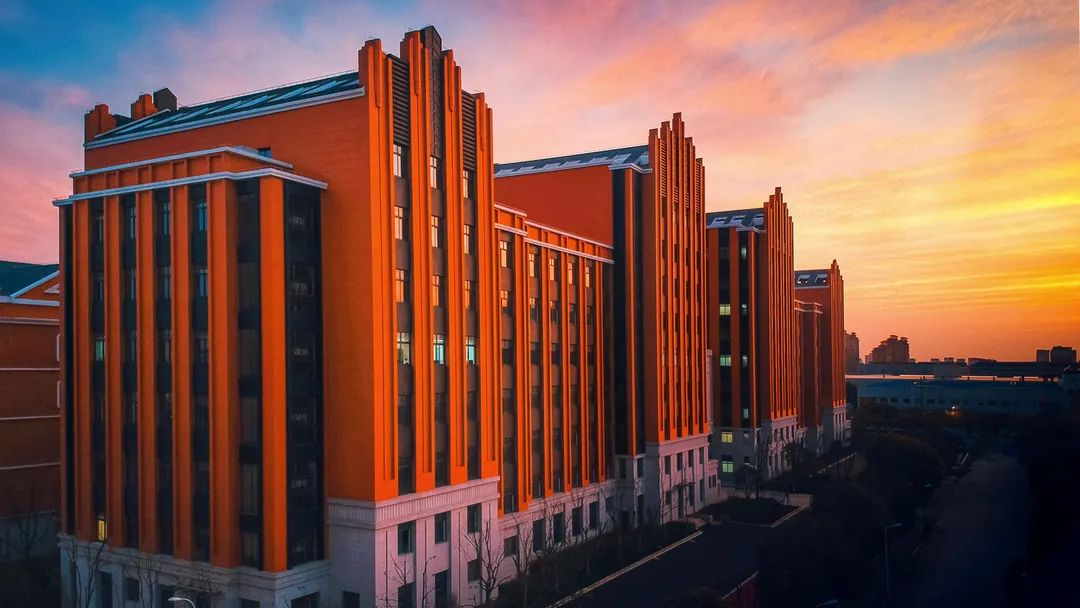
\includegraphics[width=1.5in]{img/images/img2.jpg}
                %\caption{fig1}
                \end{minipage}%
                }%
                \centering
                \subfigure[img2-RGB直方图]{
                \begin{minipage}[t]{0.5\linewidth}
                \centering
                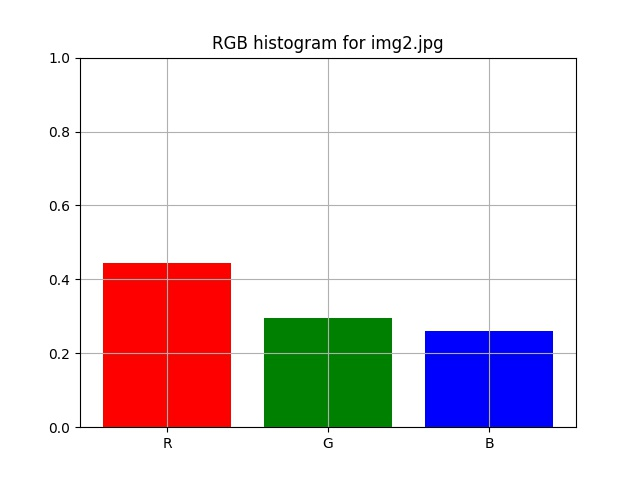
\includegraphics[width=1.5in]{img/feature/color/img2.jpg}
                %\caption{fig1}
                \end{minipage}%
                }%
            \end{figure}
            \begin{figure}[H]
                \centering
                \subfigure[img3-原图]{
                \begin{minipage}[t]{0.5\linewidth}
                \centering
                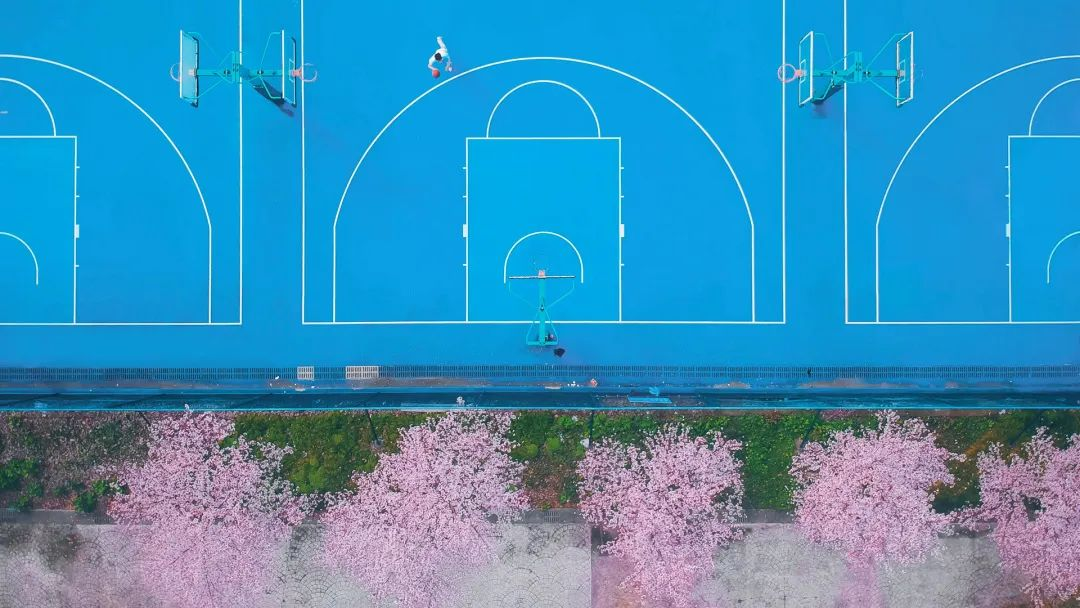
\includegraphics[width=1.5in]{img/images/img3.jpg}
                %\caption{fig1}
                \end{minipage}%
                }%
                \centering
                \subfigure[img3-RGB直方图]{
                \begin{minipage}[t]{0.5\linewidth}
                \centering
                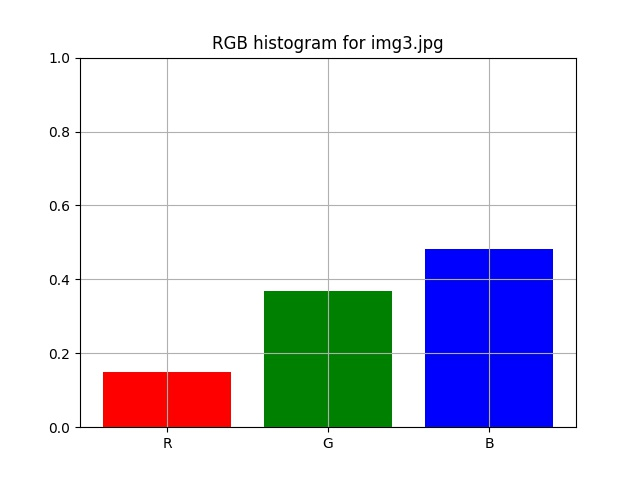
\includegraphics[width=1.5in]{img/feature/color/img3.jpg}
                %\caption{fig1}
                \end{minipage}%
                }%
            \end{figure}
        \subsection{练习二的运行结果}
            \begin{figure}[H]
                \centering
                \subfigure[img1-原图]{
                \begin{minipage}[t]{0.33\linewidth}
                \centering
                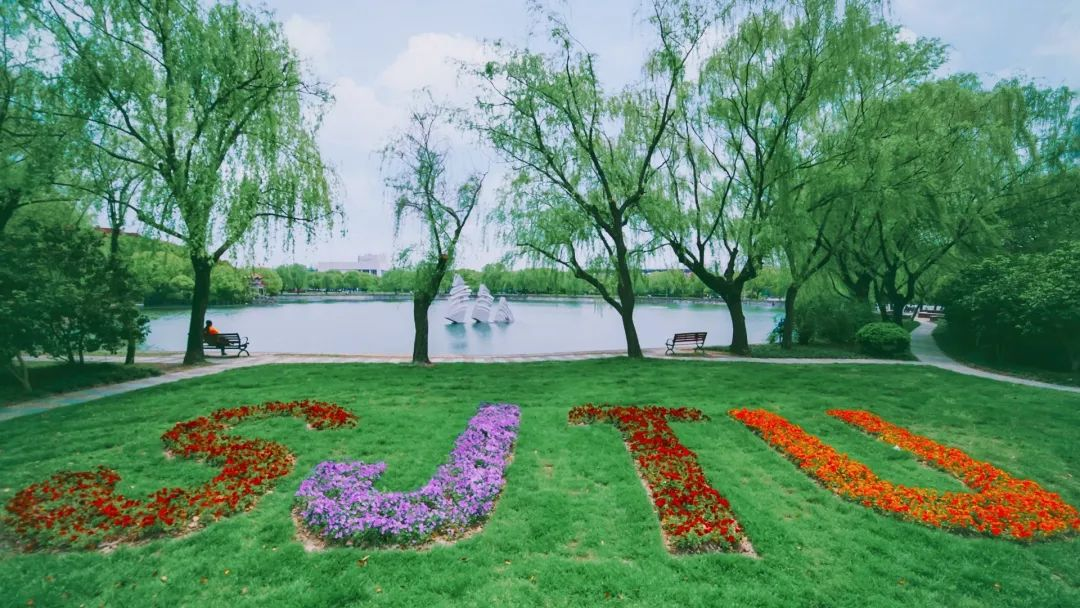
\includegraphics[width=1.3in]{img/images/img1.jpg}
                %\caption{fig1}
                \end{minipage}%
                }%
                \centering
                \subfigure[img1-灰度直方图]{
                \begin{minipage}[t]{0.33\linewidth}
                \centering
                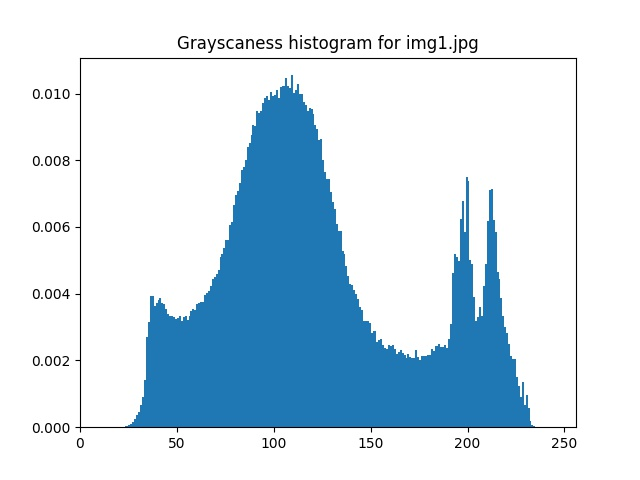
\includegraphics[width=1.3in]{img/feature/gray/img1.jpg}
                %\caption{fig1}
                \end{minipage}%
                }%
                \centering
                \subfigure[img1-灰度梯度直方图]{
                \begin{minipage}[t]{0.33\linewidth}
                \centering
                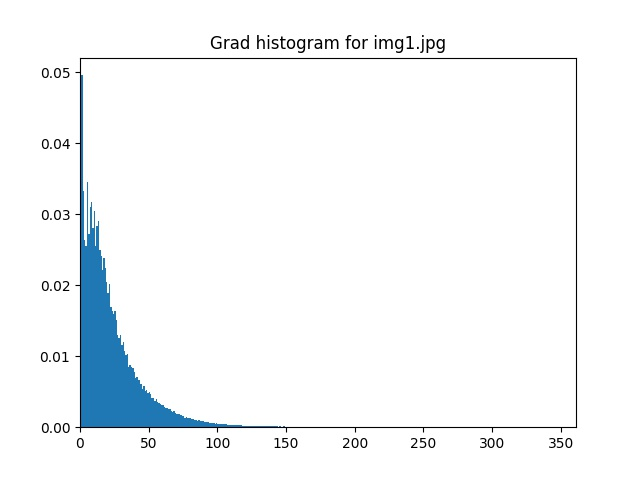
\includegraphics[width=1.3in]{img/feature/grad/img1.jpg}
                %\caption{fig1}
                \end{minipage}%
                }%
            \end{figure}
            \begin{figure}[H]
                \centering
                \subfigure[img2-原图]{
                \begin{minipage}[t]{0.33\linewidth}
                \centering
                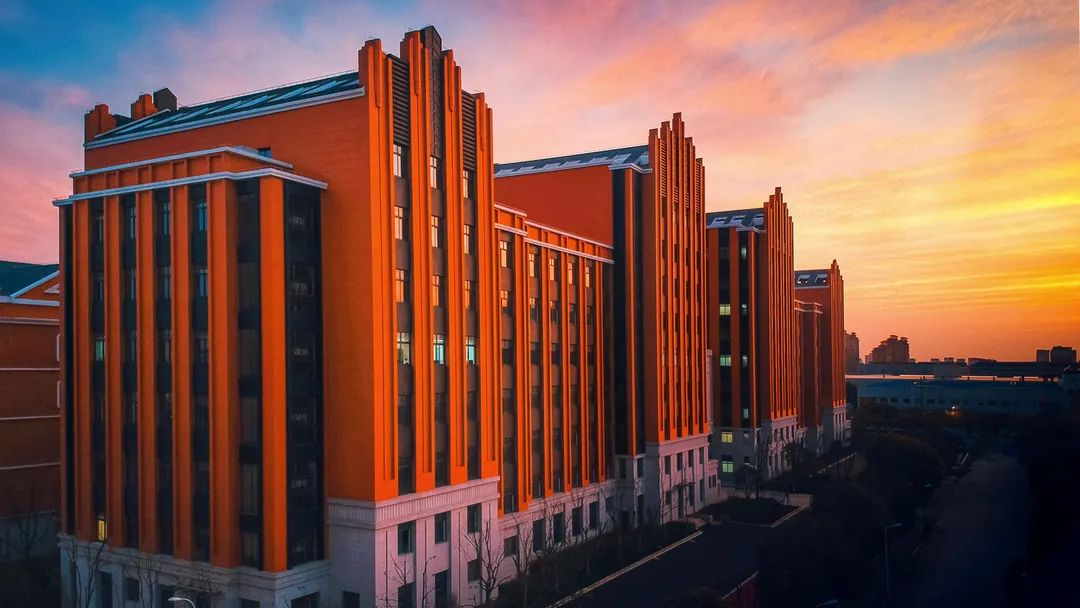
\includegraphics[width=1.3in]{img/images/img2.jpg}
                %\caption{fig1}
                \end{minipage}%
                }%
                \centering
                \subfigure[img2-灰度直方图]{
                \begin{minipage}[t]{0.33\linewidth}
                \centering
                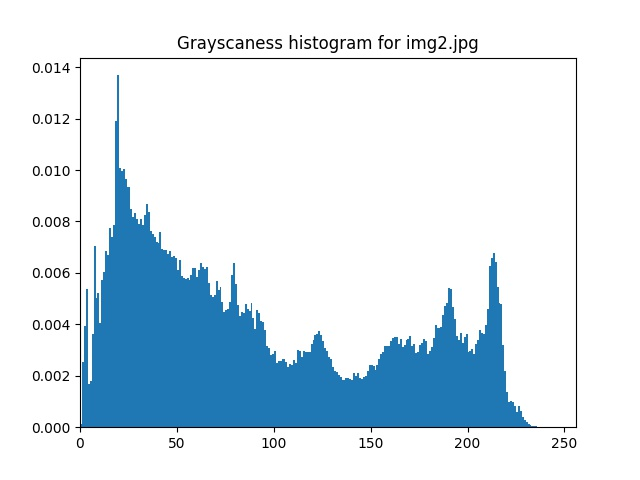
\includegraphics[width=1.3in]{img/feature/gray/img2.jpg}
                %\caption{fig1}
                \end{minipage}%
                }%
                \centering
                \subfigure[img2-灰度梯度直方图]{
                \begin{minipage}[t]{0.33\linewidth}
                \centering
                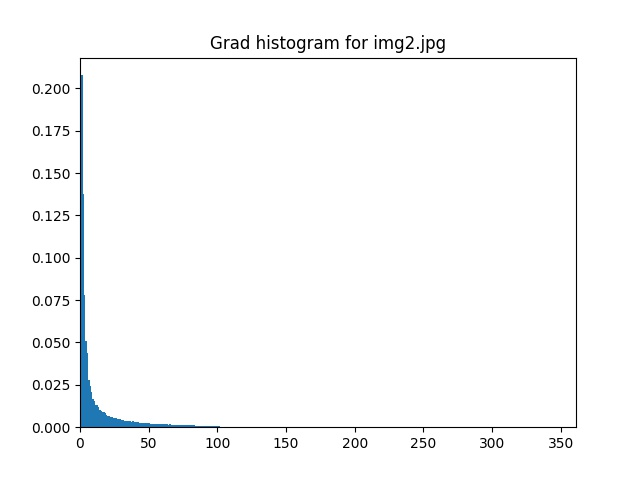
\includegraphics[width=1.3in]{img/feature/grad/img2.jpg}
                %\caption{fig1}
                \end{minipage}%
                }%
            \end{figure}
            \begin{figure}[H]
                \centering
                \subfigure[img3-原图]{
                \begin{minipage}[t]{0.33\linewidth}
                \centering
                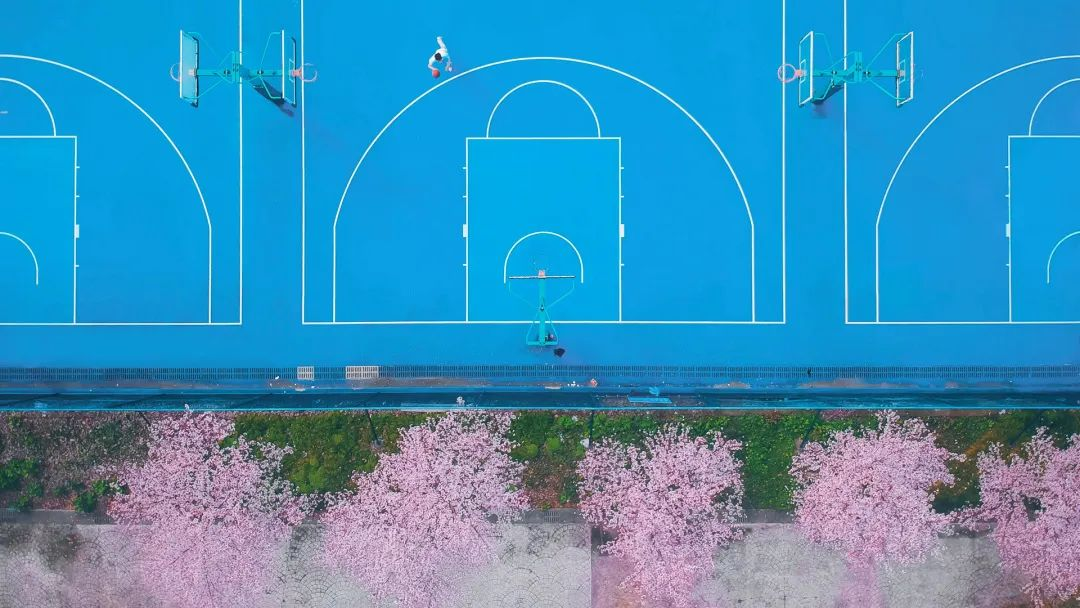
\includegraphics[width=1.3in]{img/images/img3.jpg}
                %\caption{fig1}
                \end{minipage}%
                }%
                \centering
                \subfigure[img3-灰度直方图]{
                \begin{minipage}[t]{0.33\linewidth}
                \centering
                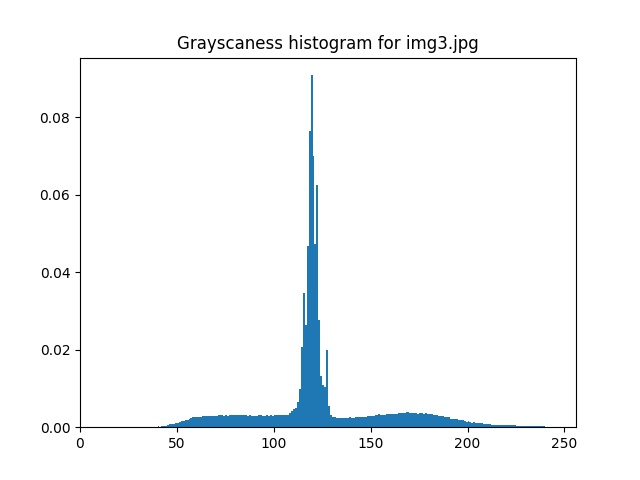
\includegraphics[width=1.3in]{img/feature/gray/img3.jpg}
                %\caption{fig1}
                \end{minipage}%
                }%
                \centering
                \subfigure[img3-灰度梯度直方图]{
                \begin{minipage}[t]{0.33\linewidth}
                \centering
                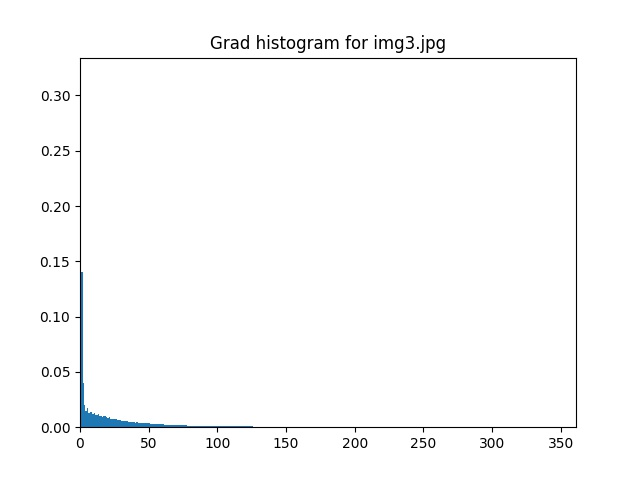
\includegraphics[width=1.3in]{img/feature/grad/img3.jpg}
                %\caption{fig1}
                \end{minipage}%
                }%
            \end{figure}
        \subsection{思考题的运行结果}
            对于思考题,对plt.imshow的函数采用不同的参数可以得到我们希望看到的灰度图的图像
            \begin{figure}[H]
                \centering
                
\includegraphics[scale=0.6]{img/show.png}
                \caption{添加参数}
            \end{figure}
            \begin{figure}[H]
                \centering
                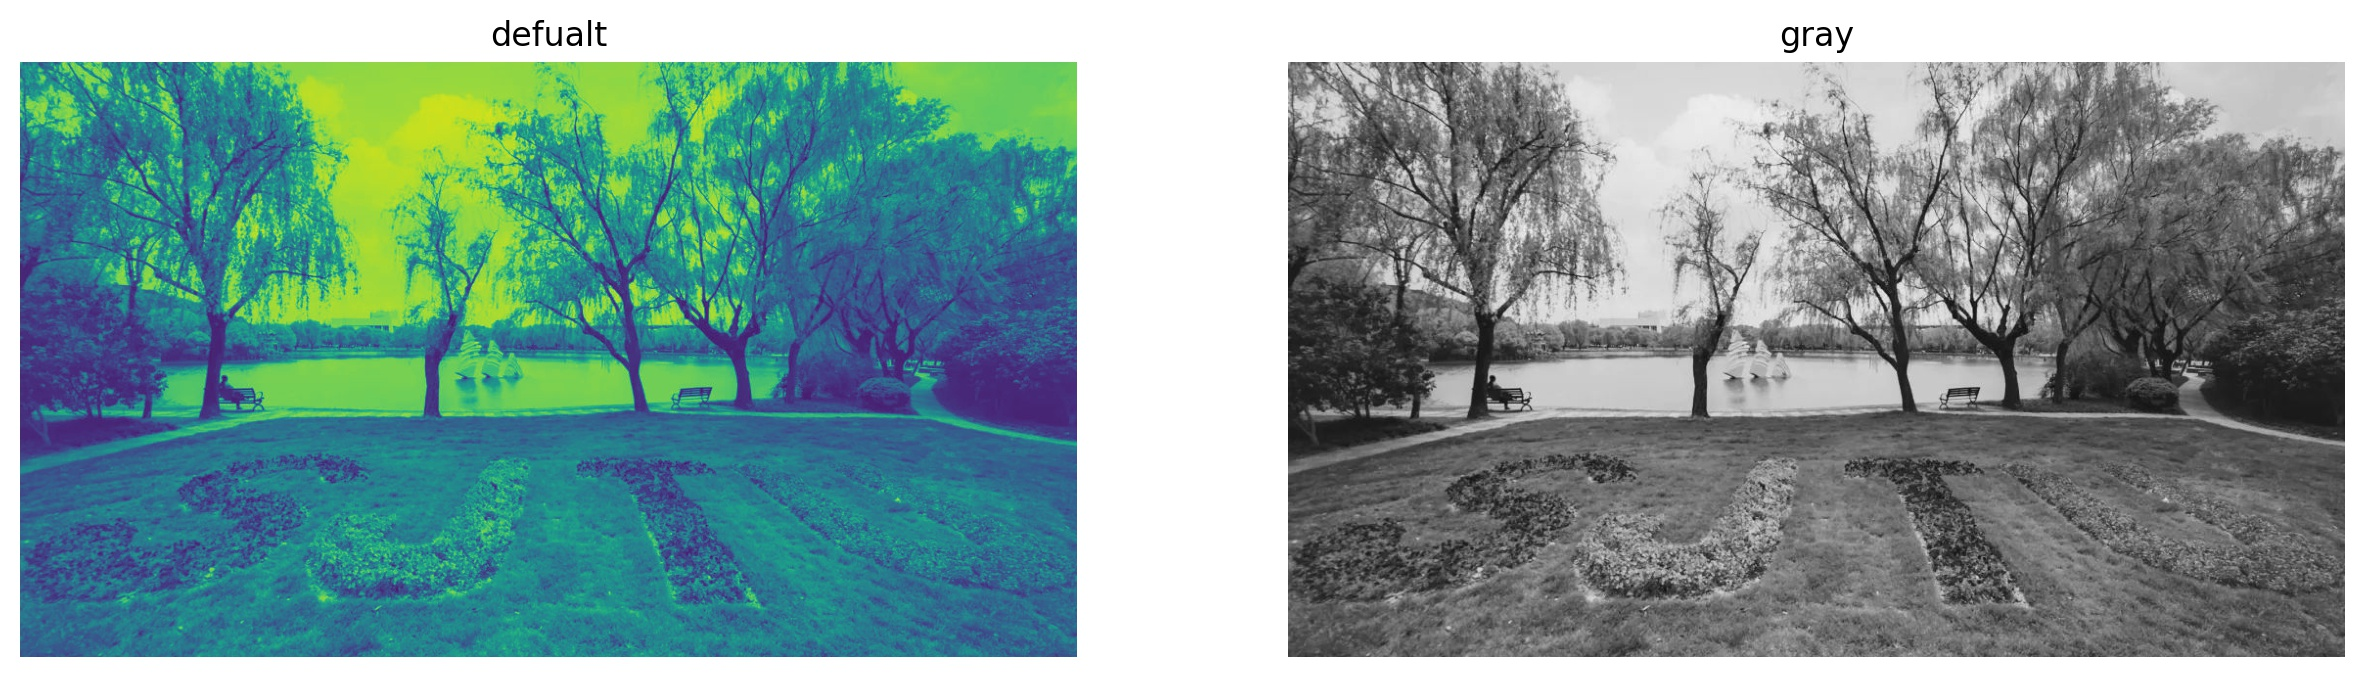
\includegraphics[scale=0.4]{img/feature/comparison.jpg}
                \caption{左图为直接显示,右图为添加了参数的结果}
            \end{figure}

    \section{思考题}
    \begin{enumerate}
        \item 由于cv2默认读取图片的方式是BGR,但plt的imshow函数又是默认进行RGB展示,所以这个函数
        是将图片从BGR模式转化为RBG式,当然,也可以通过numpy自身的切片操作来实现,具体不再赘述。本质就是将
        外层三个数组的顺序颠倒而已。
        \item 通过简单设定plt的显示参数可以进行实现,具体效果在上一个“代码运行板块中已经进行了可视化说明”
    \end{enumerate}
\end{document}